\section{\LangOO, The programming language }  
\label{s:underlying}

\subsection{\LangOO syntax runtime configurations}
\label{sub:Loo} 
{This work} is based \LangOO, a {small}, imperative, sequential,  class based, typed, object-oriented language. 
 {We believe, however, that the work can easily adapted to any capability safe language with some form of encapsulation. 
Wrt to encapsulation and  capability safety},  \LangOO supports private fields, private and public methods, unforgeable addresses, and no ambient authority (no static methods, no address manipulation).
 It has a simple concept of module with module-private fields and methods, described in Sect. \ref{sect:execution}.
 The definition of \LangOO  {can be found in the appendices  \cite{necessityFull}}, and is  similar to   OOPSLA-22.\footnoteSD{any differences?}

A \LangOO state, $\sigma$,  consists of a  heap $\chi$, and a   stack. 
{A stack  is a sequence of frames, $\phi_1\!\cdot\!...\!\cdot\! \phi_n$.}
A  frame, $\phi$, consists of a local variable map, and a continuation, \ie a sequence of statements to be executed.
%{The result of pushing a frame $\phi$ onto a stack, $\phi_1\!\cdot\!...\!\cdot\! \phi_n$, is  $\phi_1\!\cdot\!...\!\cdot\! \phi_n \!\cdot\! \phi$. }
{
The top frame in a state $(\phi_1\!\cdot\!...\!\cdot\! \phi_n, \chi)$ is $\phi_n$.} 


 
\paragraph{Notation} We adopt the following, unsurprising, notation:
\begin{itemize}
\item
{An object is uniquely identified by the address that points to it. We shall be talking of objects $o$, $o'$ when talking less formally, and of addresses, $\alpha$, $\alpha'$, $\alpha_1$, ...  when more formal.}
\item
$x$, $x'$,  ..., $y$, ... $z$, ... are variables;  $\va$, $\va'$ ... are either addresses or variables, we call these \emph{\atoms}.
\item
$\alpha \in \sigma$ means that $\alpha$ is defined in the heap of $\sigma$, and $x\in \sigma$ means that $x$ is defined in the top frame of $\sigma$.
Conversely,  $\alpha\notin\sigma$ and $x\notin\sigma$ %, and $\va \notin A$ h
 have the obvious meanings.
\item
$\interpret{\sigma}{\alpha}$  is $\alpha$; and $\interpret{\sigma}{x}$  is the value to which  $x$  is mapped in the top-most frame of $\sigma$'s stack, 
and $\interpret{\sigma}{e.f}$ looks up in $\sigma$'s heap the value of $f$ for the object  $\interpret{\sigma}{e}$.
Note that $\interpret{\sigma}{e}$ is not defined when $e$ contains a method call or a ghost field.
\item The substitution
$\phi[x \mapsto \alpha]$ is applied to the variable map  of $\phi$,  
and  $\sigma[x \mapsto \alpha]$ is applied to the top frame of $\sigma$; finally,  $\sigma[\overline{x \mapsto \alpha}]$ % applies the substitutions $\overline{x \mapsto \alpha}$ to the top frame.
has the expected meaning.
\item
%SD chipped: it does not appear later any more
%{$\phi.\prg{local\_map}$ is the local variable map of $\phi$}, 
$\phi.\prg{cont}$ is the continuation of frame $\phi$, and  $\sigma.\prg{cont}$ is the continuation in the top frame.
\item
$text_1 \txteq text_2$ expresses that $text_1$ and $text_2$ are textually equal.  
%\item  
% For statement $s_1$ and $s_2$, we write 
and $s_1 \txtin   s_2$  means  $s_1 \txteq  s_2$ or  $s_2 \txteq  s_1; s_3$ for some $s_3$, where $s_1$, $s_2$, abd $s_3$ are program statements. 
\item
{We define the depth of a stack as $\DepthFs {\phi_1...\phi_n} \triangleq n$, and for states, $\DepthSt {(\overline \phi, \chi)} \triangleq  \DepthFs {\overline \phi}$.}
\item
{ $\vs(stmt)$ returns the variables which appear in $stmt$; for example $\vs(u:=y.f)$=$\{u,y\}$.}
\end{itemize}

  

  
\subsection{\LangOO Execution}
\label{sect:execution}

%Central to our work is the distriction between the 
 \LangOO execution is described by a small steps operational semantics of the shape $\leadstoOrig  {\Mtwo} {\sigma}   {\sigma'}$.\\
  $\Mtwo$ stands for one or more modules, where a
  module,  $M$, maps class names to class definitions. 
   
{The semantics enforces dynamically a simple form of module-wide privacy: 
Fields may be read or written only if the class of the object whose field is being read or written, and the class of the object which is reading or writing belong to the same module.}
Private methods may be called only if the class of the receiver (the object whose method is being called), and the class of the caller (the object which is calling) belong to the same module.
Public methods may always be called.

The semantics is as unsurprising in all remaining aspects  :  
In $\sigma$, the  top frame's continuation contains the statement to be  executed next.  
 Statements may assign to variables, allocate new objects, 
perform field reads and writes on objects, and
 call methods on those objects. 
When a method is called, a new frame is pushed onto the stack; this frame  maps \prg{this} and the formal parameters to  the values for the receiver and other arguments, and the continuation to the body of the method.  When the continuation is ground\footnoteSD{TODO check and define}, the frame is popped and the value from the last frame's continuation is entered into the appropriate part in the caller's continuation. 
%In other aspects, the semantics is unsurprisring.%we return from that call, its frame is  popped, and execution continues in the context of the calling method. 
%The relation $\leadstoOrigStar  {\Mtwo} {\_}   {\_}$  is the reflexive, transitive closure of $\leadstoOrig  {\Mtwo} {\_}   {\_}$ .


{Fig. \ref{fig:UpSemantics} illustrates  such  execution steps:  disks indicate states;
 horizontal $\leadstoN$-arrows denote   steps  within the same  call; upwards arrows denote  method calls;
 %(pushing a new frame onto the stack);  
 downwards arrows denote method returns. % (popping the top of the stack). 
 Here,   $\leadstoOrig {\Mtwo}{\sigma_8}   {\sigma_9} $ is a step within the same call, $\leadstoOrig {\Mtwo}{\sigma_9}   {\sigma_{10}} $ is a method call   
with $\leadstoOrig {\Mtwo}{\sigma_{12}}   {\sigma_{13}} $ %is a method return  (from the call to $m_a$), 
the corresponding return. 
 {Note that  $\leadstoOrigStar  {\Mtwo} {\sigma}   {\sigma'}$ may involve  any number of  calls or returns: 
 $\leadstoOrigStar  {\Mtwo} {\sigma_8}   {\sigma_{12}}$ involves one call and no return,
while $\leadstoOrigStar  {\Mtwo} {\sigma_{10}}   {\sigma_{15}}$,   involves no calls and two returns.
% In section \ref{sect:bounded}, we will define a derived relation, called bounded execution, where the number of returns may not exceed the number of calls.
}
} 

\begin{figure}[htb]
\begin{tabular}{|c|}
 \hline %  \\ -- this added one vertical space
\resizebox{7cm}{!}{
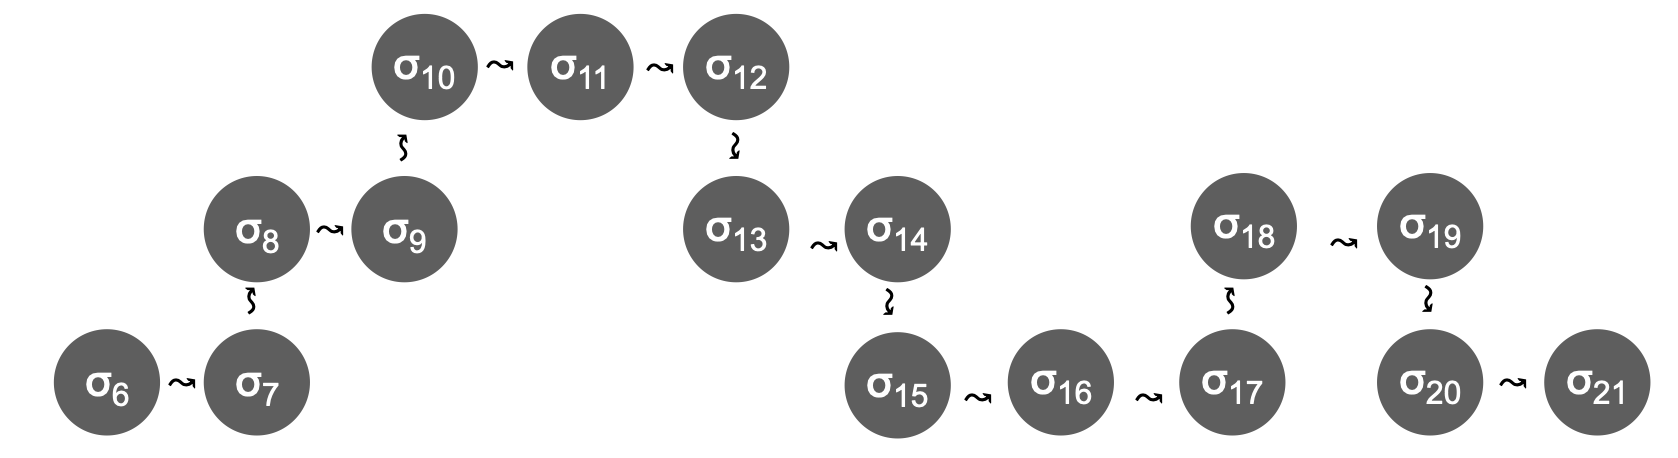
\includegraphics[width=\linewidth]{diagrams/bounded.png}
} 
 \\
\hline

\end{tabular}
   \caption{Illustrating   $\leadstoOrig  {\Mtwo} {\sigma}    {\sigma'}$ 
    }
   \label{fig:UpSemantics}
 \end{figure}
 
%\susan{I don't think the two lines at the bottom of the figure are needed here and in the next figure. {agree, but highlight.}} 
 
%{Note that $\leadstoOrig {\Mtwo}{\sigma_{8}}   {\sigma_{9}} $ and $\leadstoOrig {\Mtwo}{\sigma_{13}}   {\sigma_{14}} $ are steps within the same call, but 
%$\leadstoOrig {\Mtwo}{\sigma_{14}}   {\sigma_{15}} $ and $\leadstoOrig {\Mtwo}{\sigma_{17}}   {\sigma_{18}} $ are not. %steps within the same call,
%% even though all four states ($\sigma_{13}$, $\sigma_{14}$, $\sigma_{17}$, and $\sigma_{18}$), have the same number of frames on their stack.
%We want a semantics to reflect whether execution steps happen within the bounds of certain call. For this, we define \emph{bounded execution}, 
%$\leadstoBounded {\Mtwo} {\sigma} {\sigma''} {\sigma'}$ 
%which are execution steps which lead from $\sigma$ to $\sigma'$ while not popping  $\sigma''$-s top frame.
%This will be defined in Section \ref{sect:bounded}.
%}

%\subsection*{Applicability} 
%While our work is based on the particular language  \LangOO , % a simple, imperative, typed, object oriented  language with unforgeable addresses and private fields, we believe that % our approach
%we believe that it is applicable to several programming paradigms, and  that   unforgeability and privacy
% can be replaced  by lower level mechanisms such as capability machines \cite{vanproving,davis2019cheriabi}.


\section{Auxiliary concepts}
\label{s:auxiliary}

{To develop the semantics of our assertions language, \AssertLang, we   \sdN{define} three auxiliary, \sdN{derived}, concepts on  top of  \LangOO: scoped execution, method calls and returns, and reachable objects.}

\subsection{ Method Calls and Returns}

 
 
Method calls and returns are a fundamental concern for our work. 
They are characterized through pushing/popping   frames on the stack.  
The operator   $ \PushS  {\phi} {\sigma}$ pushes 
frame $\phi$ onto the stack of $\sigma$.
 
 

\begin{definition}
\label{def:push:frame}
Given a state $\sigma$, addresses $\overline \alpha$, a frame $\phi$,  variables or addresses $\overline \va$, we define
\begin{itemize}
\item
 $ \PushSF  {\phi} {\sigma} \ \triangleq \ ({\overline{\phi}\cdot\phi}, \chi)$ \ \ \  if \ \ \  $\sigma=(\overline{\phi}, \chi)$.
\item
$ \PushS  {\alpha} {\sigma} \ \triangleq\ \{ \ \sigma' \ \mid\ \exists \phi  \ s.t.\ \ 
   \sigma'=\PushSF  {\phi} {\sigma}  \ \wedge\    Rng(\phi)=\overline \alpha \ \   \ \}$
\item
{$ \PushS  {\va}  {\sigma}\  \triangleq\     \PushS  {\interpret {\sigma} {\va}} {\sigma} $.}
\item
$ \sigma\, \popSymbol \ \ \  \triangleq\   \sdN{ (\overline{\phi}\cdot (\phi_n[\prg{cont}\mapsto stmt][x \mapsto \interpret {\phi_n}{ret}]), \chi)}$ \ \ \  if \\
 $\strut \hspace{1.2cm}  \exists x, y_0, \overline y. [ \ \sigma=(\overline{\phi}\cdot\phi_n\cdot\phi_{n+1}, \chi)$, and $\phi_n(\prg{cont})\txteq x:= y_0.m(\overline y); stmt \ ]$
\end{itemize}
 \end{definition}
\footnoteSD{\red{DO we also need that $\overline \alpha$ were locally reachable in $\sigma$?}}

Consider Fig. \ref{fig:UpSemantics} again: $\sigma_8\!\in\!   \PushS  {\phi} {\sigma_7}$ for some $\phi$ -- {thus $\sigma_8$ is a callee state for 
 $\sigma_7$}. {And $\sigma_{15}$=$\sigma_{14} \popSymbol$ --  thus $\sigma_{15}$ is the return state from 
 $\sigma_{14}$.}
% Note that $\sigma = \sigma' \popSymbol$ iff $\sigma'\!\in\!\PushS  {\phi} {\sigma}$; we can see that 
% Also, 
% $\sigma_{14}\!\in\!\PushS  {\phi'} {\sigma_{15}}$ for some $\overline {\alpha'}$ -- {thus $\sigma_{15}$ is a caller state for  $\sigma_{14}$}.
%\footnote{$\phi'$ may differ from $\phi$, because between $\sigma_8$ and $\sigma_{15}$ there may 
% have been assignments to local variables.} 

  
 \subsection{Scoping}
 \label{sect:bounded}

{The semantics from the earlier section allows arbitrary numbers of method calls and returns. 
In particular, it is possible to start with a state $\sigma$ and perform more returns than calls --
\eg $\leadstoOrigStar  {\Mtwo} {\sigma_{8}}   {\sigma_{15}}$  in  Fig. \ref{fig:UpSemantics}.
{In the sense of $\rightarrow^*$,  the state $\sigma_{15}$  is one of the future  states for $\sigma_8$.}

 
{For} the purposes of our work, we   need an {additional} notion, of  \emph{scoped} future:  
the scoped future of a state consists of all states which  can be reached through any   
 steps, including method calls and returns, but   {stopping before returning}   
from the method executing in the scoping state}. 
\forget{We say the currently executing method \emph{scopes} the execution.}
Thus, the {scoped} future  of $\sigma_8$   includes only
  $\sigma_9$, $\sigma_{10}$, $\sigma_{11}$, $\sigma_{12}$, $\sigma_{13}$, and $\sigma_{14}$, but \emph{not} $\sigma_{15}$  -- the latter results from returning from $\sigma_{8}$'s top continuation.  
 {Similarly, $\sigma_{18}$ is not in the scoped future of $\sigma_8$, even though the two states have the same stack depth -- between $\sigma_{8}$  and  $\sigma_{18}$ we returned from the top continuation in $\sigma_{8}$.}
 
 

To capture this  notion, we define    {\emph{execution scoped by a state} $\sigma\bd$, which  allows any steps, except for popping   $\sigma\bd$'s top frame:}
 
 
\begin{definition}[Scoped Execution]
\label{def:shallow:term}
We define relations \    $\leadstoBoundedThree {\Mtwo} {\sigma} {\sigma\bd} {\sigma'}$ \ and\  $\leadstoBounded  {\Mtwo} {\sigma} {\sigma'}$ as:

\begin{itemize}
\item
 $\EarlierS {\sigma}  {\sigma'} \ \ \ \ \ \  \ \ \ \ \ \ \ \ \ \  \ \ \  \triangleq \ \ % \exists  \psi, \psi', s.t. 
 {\exists  \phi, \phi',\overline \phi, \overline {\phi'} [\  \sigma\!=\!({\overline \phi\cdot \phi},\_)\, \wedge\, \sigma'\!=\!(\overline \phi\cdot \phi'\cdot \overline {\phi'},\_)\ ] } $\footnote{Needless to say that   $\overline \phi$ as well as ${\overline {\phi'}}$ may be empty.}
 %\ \  \vee\  \ 
 %\exists \phi,\sigma''.[\  \EarlierS {\sigma} {\sigma''}\,  \wedge\,  \sigma'\!=\!\PushSF {\phi} {\sigma''}\ ]$ 
\item
{ $\leadstoBoundedThree {\Mtwo} {\sigma} {\sigma\bd}  {\sigma'}  \  \   \triangleq \ \    \leadstoOrig {\Mtwo} {\sigma} {\sigma'} \, \wedge\, 
 \EarlierS {\sigma\bd}  {\sigma} \, \wedge\,  \EarlierS {\sigma\bd}  {\sigma'} $}
\item
 $\leadstoBoundedStarThree  {\Mtwo}  {\sigma}  {\sigma\bd} {\sigma'} \ \ \ \triangleq \ \  \sigma=\sigma' \, \wedge\,  \EarlierS {\sigma\bd}  {\sigma}\  \ \ \vee
 % $\\ $\strut  \hspace{3cm}\
 \ \ \ \exists \sigma''.[\ \leadstoBoundedThree  {\Mtwo}  {\sigma}  {\sigma\bd} {\sigma''} \, \wedge\, 
\leadstoBoundedStarThree {\Mtwo} {\sigma''} {\sigma\bd}  {\sigma'}\ ]$
 \item
{  $\leadstoBounded  {\Mtwo} {\sigma}   {\sigma'} \ \  \ \ \ \ \   \,   \ \ \ \triangleq \ \ \  \leadstoBoundedThree {\Mtwo} {\sigma} {\sigma}  {\sigma'}$}
  \item
{  $\leadstoBoundedStar {\Mtwo}  {\sigma}  {\sigma'}   \ \ \ \ \ \ \,  \ \ \ \  \ \triangleq  \ \ \  \leadstoBoundedStarThree {\Mtwo}  {\sigma}  {\sigma} {\sigma'}$}\ \  
\item
  $\leadstoBoundedStarFin {\Mtwo}  {\sigma}  {\sigma'}   \ \ \ \ \  \,  \ \  \ \triangleq  \ \ \  \leadstoBoundedStar {\Mtwo}  {\sigma}  {\sigma'}  \ \wedge\ \
 {\DepthFs \sigma = \DepthFs {\sigma'} \ \ \wedge \ \ \sigma'.\prg{cont}=\epsilon  } $
%  \neg[\ \exists \sigma''.\ \leadstoBoundedThree {\Mtwo} {\sigma'}  {\sigma} {\sigma''} \ ]$ }
 \end{itemize}
\end{definition}


We continue with  Fig. \ref{fig:UpSemantics}. {Here $\EarlierS {\sigma_8} {\sigma_9}$ and thus $\leadstoBoundedThree {\Mtwo} {\sigma_8} {\sigma_8} {\sigma_9}$.} Also,  {$\leadstoOrig {\Mtwo} {\sigma_{14}}  {\sigma_{15}}$ 
 but  {$\NotEarlierS {\sigma_{14}} {\sigma_{15}} $} and therefore  $\notLeadstoBoundedThree {\Mtwo}  {\sigma_{14}} {\sigma_{14}} {\sigma_{15}}$ and $\notLeadstoBounded  {\Mtwo}  {\sigma_{14}}   {\sigma_{15}}$
--  this step would pop  $\sigma_{14}$'s
 top frame. 
% Therefore,   $\leadstoOrigStar {\Mtwo} {\sigma_8}  {\sigma_{15}}$ 
%  but  $\notLeadstoBoundedStarThree {\Mtwo} {\sigma_8} {\sigma_8} {\sigma_{15}}$, and  $\notLeadstoBoundedStarThree {\Mtwo}  {\sigma_8} {\sigma_{15}}$.
 Also, $\leadstoOrigStar {\Mtwo} {\sigma_8}  {\sigma_{18}}$ 
 but  $\notLeadstoBoundedStar {\Mtwo} {\sigma_8}   {\sigma_{18}}$  -- even though $\sigma_8$ and $\sigma_{18}$ have the same depth of stack, they belong to different calls. 
 {In particular, $\NotEarlierS {\sigma_{8}} {\sigma_{15}} $, and thus 
 $\notLeadstoBoundedThree {\Mtwo} {\sigma_{14}} {\sigma_8}   {\sigma_{15}}$ -- this is the step that would correspond  to popping the top stack frame from $\sigma_8$.}

 \move{ 
Lemma \ref{lemma:orig:to:bounded}  states that
 any execution  which is part of an execution which started at some initial state, is scoped by that state.
%\ (\ref{otbOne})\  Any state in the future of some  initial state is in the  scoped future   of that state.
%\ (\ref{otbTwo})\ %  
% {If a state $\sigma$ is in the future of some initial state $\sigma_{init}$, then any execution from $\sigma$ to $\sigma'$  is scoped by   $\sigma_{init}$.}
%While an execution from $\sigma$ to $\sigma'$ need not be scoped ($\leadstoOrigStar {\Mtwo} {\sigma}  {\sigma'}$ does not imply $ \leadstoBoundedStar {\Mtwo} {\sigma}  {\sigma'}$), 
%if $\sigma$ is in the future of some initial state $\sigma_{init}$, then $\sigma$ is reachable from some initial state $\sigma_{init}$
% then $\sigma_{init}$  bounds the execution from $\sigma$ to   $\sigma'$. 
% \ (\ref{otbThree})\  generalizes %  Lemma \ref{lemma:orig:to:bounded},  part
% (\ref{otbTwo}): {For any execution starting at some initial state $\sigma_{init}$ and leading from $\sigma_m$ to $\sigma_n$, 
% we can find $\sigma_k$, a predecessor of $\sigma_m$, which  scopes the execution from $\sigma_m$ to $\sigma_n$; moreover all
%  predecessors  for $\sigma_k$ scope that execution, while its successors do not.}
% % there exists a further, earlier, state $\sigma_o$, such that both $\sigma$ and $\sigma'$ are  
%%part   of $\sigma_o$'s bounded future. Moreover, from $\sigma_o$'s viewpoint, $\sigma'$ is a transitive bounded successor of $\sigma$.}
%Bounded semantics impose restrictions on the set of future states, but only from the viewpoint of {the bounding} \susan{binding?%\red{SD: I thought that binding goes with "bind" and "bounding" goes with "bounded" -- i.e., the state that provides the bound}} state. 
\forget{
Lemma \ref{lemma:orig:to:bounded}  states that:  
\ (\ref{otbOne})\  All executions starting at an initial state  are in scope.
\ (\ref{otbTwo})\  {While an execution from $\sigma$ to $\sigma'$ need not be in scope  ($\leadstoOrigStar {\Mtwo} {\sigma}  {\sigma'}$ does not imply $ \leadstoBoundedStar {\Mtwo} {\sigma}  {\sigma'}$), if $\sigma$ is in the scoped future of some initial state $\sigma_{init}$, 
 then $\sigma_{init}$  scopes the execution from $\sigma$ to   $\sigma'$. }
 \ (\ref{otbThree})\  generalizes %  Lemma \ref{lemma:orig:to:bounded},  part
 (\ref{otbTwo}): {For any execution starting at some initial state $\sigma_{init}$ and leading from $\sigma_m$ to $\sigma_n$, 
 we can find $\sigma_k$, a predecessor of $\sigma_m$, which  scopes the execution from $\sigma_m$ to $\sigma_n$; moreover all
  predecessors  for $\sigma_k$ scope that execution, while its successors do not.}
  }
 % there exists a further, earlier, state $\sigma_o$, such that both $\sigma$ and $\sigma'$ are  
%part   of $\sigma_o$'s bounded future. Moreover, from $\sigma_o$'s viewpoint, $\sigma'$ is a transitive bounded successor of $\sigma$.}


 \begin{lemma}
\label{lemma:orig:to:bounded}
For all $\overline M$, all $n,m\in \mathbb{N}$ with $m\leq n$, $\sigma_0$, ... $\sigma_n$,  $\sigma_{init}$, $\sigma$, $\sigma'$, where
$\sigma_{init}$ is an initial state:\footnote{An \emph{Initial} state's heap contains a single object of class \prg{Object}, and
its  stack   consists of a single frame, whose local variable map is a mapping from \prg{this} to the single object, and whose continuation is  any statement.
(See Definition %s \ref{def:initial} and 
\ref{def:arising} and the 
{appendices %of the full paper 
\cite{necessityFull}).}} 
\begin{itemize} % {enumerate} 
%\item 
%\label{otbOne}
%$\leadstoOrigStar {\Mtwo} {\sigma_{init}}  {\sigma}\ \ \Longrightarrow\ \  \leadstoBoundedStar {\Mtwo}  {\sigma_{init}} {\sigma}$.
\item 
\label{otbTwo}
$\leadstoOrigStar {\Mtwo} {\sigma_{init}}  {\sigma}\ \wedge\ \leadstoOrigStar {\Mtwo} {\sigma}  {\sigma'}\ \ \Longrightarrow\ \  \leadstoBoundedStarThree {\Mtwo} {\sigma} {\sigma_{init}} {\sigma'}$.
%there exists a $\sigma_o$, such that $\leadstoBoundedStar {\Mtwo} {\sigma_{init}}  {\sigma_o}$, and
% $\leadstoBoundedStar {\Mtwo} {\sigma_o}  {\sigma}$, and $\leadstoBoundedStar {\Mtwo} {\sigma_o}  {\sigma'}$, and $\leadstoBoundedStar {\Mtwo} {\sigma_o}  {\sigma'}$. More specifically, 
% $\leadstoBoundedStarThree {\Mtwo} {\sigma} {\sigma_o} {\sigma'}$.
%\item
%\label{otbThree}
% $\forall i\!\in\! [0..m).\ \leadstoOrig  {\Mtwo} {\sigma_{i}}  {\sigma_{i+1}}\ \wedge\ \sigma_{init}=\sigma_0$ \\
% % \ \wedge \  \sigma=\sigma_m \ \wedge\ \sigma' =\sigma_n  $ \\
%\strut \hspace{0.5cm} $\ \ \Longrightarrow \ \  \exists k\leq m.[\ \ \ \forall i\leq k.[\  % \leadstoBoundedStar  {\Mtwo}   {\sigma_{init}} {\sigma_i}\ \wedge \ 
%\leadstoBoundedStarThree  {\Mtwo}  {\sigma_m}  {\sigma_{i}} {\sigma_n} ]\ \ \  \wedge \ \ \ 
%% $\\ \strut \hspace{3cm} $
% \forall i> k. [\  \notLeadstoBoundedStarThree  {\Mtwo}  {\sigma_m}  {\sigma_{i}} {\sigma_n}\ ] \ \ \ ]$.
%\end{enumerate} 
\end{itemize}
\end{lemma}
 



{Revisit  Fig. \ref{fig:UpSemantics}, and assume that $\sigma_6$ is an initial state.
We have  $\leadstoOrigStar {\Mtwo} {\sigma_{10}}  {\sigma_{14}}$ and $ \notLeadstoBoundedStar {\Mtwo}  {\sigma_{10}} {\sigma_{14}}$.
However, because $\sigma_6$ is an initial state, we have $\leadstoBoundedStarThree {\Mtwo}  {\sigma_{10}} {\sigma_{6}}  {\sigma_{14}}$ -- \cf Lemma \ref{lemma:orig:to:bounded}.
% SD chopped as we removed that part of lemma
%Moreover, we have that  $\forall i\in [6..9].\leadstoBoundedStarThree {\Mtwo}  {\sigma_{10}} {\sigma_{i}}  {\sigma_{14}}$ -- part (\ref{otbThree})  from above. 
}}

\se{Finally,} Lemma \ref{l:var:unaffect} says that the interpretation of a variable remains unaffected by scoped execution of statements  which do not mention that variable.

\begin{lemma}
\label{l:var:unaffect}
For any modules $\Mtwo$, states $\sigma$, $\sigma'$, and variable $y$ 
\begin{itemize}
\item
$\leadstoBoundedStarFin {\Mtwo}  {\sigma}  {\sigma'} \ \wedge \ y\notin \vs(\sigma.\prg{cont}) \ \ \Longrightarrow \ \  \interpret \sigma y =  \interpret {\sigma'} y$
\end{itemize}

\end{lemma}

\move{
Finally, Lemma \ref{lemma:call:return}
states that method calls  correspond  to pushing of frames (here $\sigma_2 \in \PushS  {\interpret {\sigma_1} {y}} {\sigma_1}$),
 that they leave the values of the caller's local variables unmodified ($\forall z. \interpret {\sigma_1} {z} = \interpret {\sigma_4} {z}$), and
method returns  correspond  to popping  a frame  (here $\sigma_3 \in  \PushSLong  {( {\interpret {\sigma_1} {y}},{\overline \alpha})} {\sigma_4}$), where the local map of the frame being popped contains the original arguments ($\overline {{\interpret {\sigma_1} {y}}}$) as well as some additional addresses ($\overline \alpha$).
The latter property -- that  the frame being popped from $\sigma_3$ contained the original arguments passed in to $\sigma_2$ -- holds because 
 we forbid assignments to formal parameters (but we do allow  assignments to the other local variables).
 
 
 \begin{lemma}
 \label{lemma:call:return}
 For any modules $\Mtwo$, states $\sigma_1$, $\sigma_2$, $\sigma_3$, and $\sigma_4$, variables $x$, $y_0... y_n$:
% \\
% If  $\sigma_1.\prg{cont}\txteq x:= y_0.m(y_1,...y_n);\_$, and $\leadstoOrig {\Mtwo} {\sigma_1}   {\sigma_2} $ and 
% $\leadstoBoundedStarFin  {\Mtwo}  {\sigma_2}  {\sigma_3}$, and $\leadstoOrig {\Mtwo} {\sigma_3}   {\sigma_4} $, then
% \\
% $\sigma_2 \in \PushS  {\interpret {\sigma_1} {y}} {\sigma_1}\ \wedge\  \forall i. \interpret {\sigma_1} {y_i} = \interpret {\sigma_4} {y_i}\ \wedge\  \exists \overline \alpha. [\ \sigma_3 \in  \PushSLong  {( {\interpret {\sigma_1} {y}},{\overline \alpha})} {\sigma_4} \ ]$
 
 $  
   \left. %\{
   \begin{array}{l}  \ \strut \ \ \sigma_1.\prg{cont}\txteq x:= y_0.m(y_1,...y_n);\_ ,\\
    \ \strut \ \  \leadstoOrig {\Mtwo} {\sigma_1}   {\sigma_2} , \\
     \ \strut \ \  \leadstoBoundedStarFin  {\Mtwo}  {\sigma_2}  {\sigma_3}, \\
  \ \strut \ \  \leadstoOrig {\Mtwo} {\sigma_3}   {\sigma_4}, 
    \end{array} 
\right \}
 \mbox{implies} \ \ 
  \begin{cases}
     \ \strut \ \  \sigma_2 \in \PushS  {\interpret {\sigma_1} {y}} {\sigma_1},\\
     \ \strut \  \exists z.\ \sigma_3.\prg{cont}{\txtin z} \\
       \ \strut \ \       \forall z. \interpret {\sigma_1} {z} = \interpret {\sigma_4} {z},\\  
        \ \strut \ \       \exists \overline \alpha. [\ \sigma_3 \in  \PushSLong  {( {\interpret {\sigma_1} {y}},{\overline \alpha})} {\sigma_4} \ ]
    \end{cases} 
$
 \end{lemma}

}
  \subsection{{{Locally} Reachable  Objects}}

 {A central concept to our work is %object 
protection, which we will define in   Sect. \ref{sect:protect}: It requires that no external locally reachable object  
%reachable from the top frame  
can have unmitigated access to that object.}
%
%{The  \SpecLang  specifications support universal quantification over  objects; such specifications 
%are applicable  to all objects in the heap witch, are however, either locally reachable (i.e. there is in the heap a path from the an 
%object on the top frame to the particular object), or globally reachable (i.e. there is in the heap a path from the an 
%object on some frame to the particular object.)
%%In this section  we will formally define these concepts.}\footnoteSD{TODO we need a better motivation for these concepts.}
%
An object $\alpha$ is  locally reachable, $ \LRelevant \alpha \sigma $, if it is reachable from the top frame on the stack of $\sigma$.
% SD dropped the below, as we do not use it,
%and it is globally reachable, $\GRelevant \alpha \sigma$, if it is reachable from any  frame on the stack of $\sigma$.
 
\begin{definition} We define 
\begin{itemize}
\item
$ \LRelevant \alpha \sigma $ \ \ iff\ \  
$\exists \phi.[\ \sigma=(\phi\cdot\_, \_)$ and $\Relevant \alpha \phi \sigma\ ]$. % for some $\phi$
%\item
%$\GRelevant \alpha \sigma$  \ \ iff\ \  
%$\exists \phi.[\ \sigma=(\_\cdot\phi\cdot\_, \_)$ and $\Relevant \alpha \phi \sigma\ ]$. % for some $\phi$
\end{itemize}
where\\
$\strut\ \ \ \  \ \ \ \ \ \ \Relevant \alpha \phi \sigma $  \ \ \ \ \ \ \ iff\ \  
$\exists n\in \mathbb{N}.\exists \prg{f}_1,... \prg{f}_n.\exists \prg{x}.[ \ \interpret{\sigma}{\phi(x).\prg{f}_1.....\prg{f}_n} = \alpha \ \ ]$.

\end{definition}

 \begin{figure}[htb]
\begin{tabular}{|c|c|c|}
\hline \\
\resizebox{3.5cm}{!}{
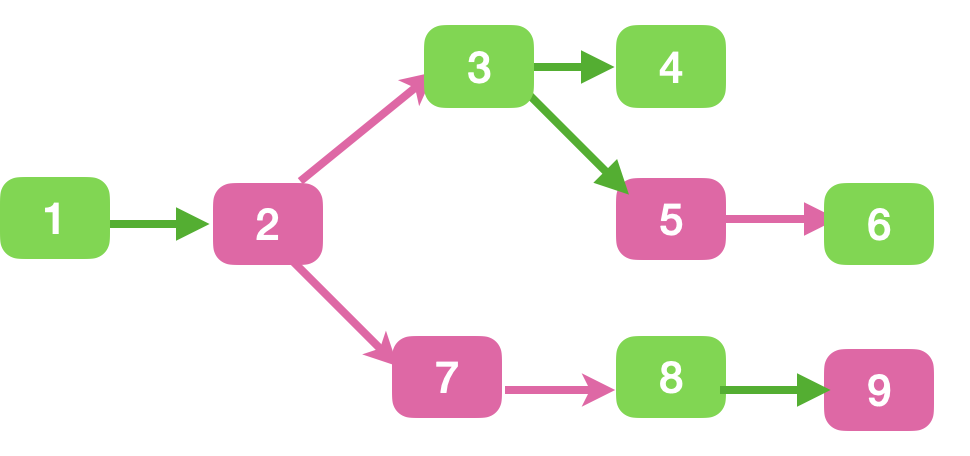
\includegraphics[width=\linewidth]{diagrams/heap.png}
} 
&
\resizebox{5cm}{!}{
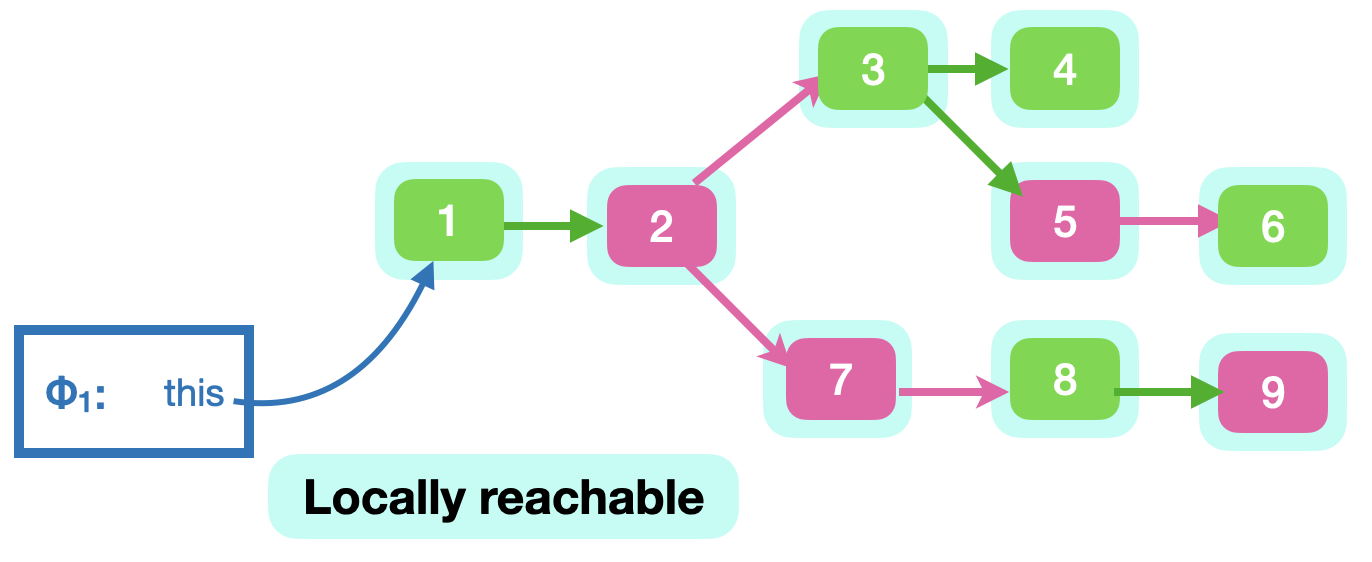
\includegraphics[width=\linewidth]{diagrams/locReachA.png}
} 
&
\resizebox{5cm}{!}{
\includegraphics[width=\linewidth]{diagrams//locReachb.png}
} 
\\
\hline
 a heap
&
Locally Reachable from $\phi_1$
&
Locally Reachable from $\phi_2$
\\
\hline \hline
\end{tabular}
   \caption{A heap, two stacks, and Locally Reachable Objects.
  Distinction  objects into  green/pink  explained later. } % from $\phi_1$ and $\phi_2$. } % n later chapters}
   \label{fig:LReachable}
 \end{figure}

We illustrate these concepts in Fig. \ref{fig:LReachable}:  In the middle pane the top frame is $\phi_1$ which maps \prg{this} to $o_1$; all objects are locally reachable. 
In the right pane the top frame is $\phi_2$, which maps \prg{this} to $o_3$, and $x$ to $o_7$; now $o_1$ and $o_2$ are no longer locally reachable.

Lemma  \ref{lemma:relevant} % describes properties of global reachability. 
says that 
% SD removed globally reachable
% (\ref{oneGR}) Locally reachable objects are globally reachable. 
%(\ref{twoGR}) 
%% Any object which will be globally reachable at some future state  and which exists object in the current state, is globally reachable the current state: that is, 
%Globally unreachable objects may not become reachable in the future.
(\ref{threeLR}) A pre-existing object, locally reachable after any number of scoped execution steps, was locally reachable at the first step.
\footnoteSD{cite "only connectivity begets connectivity"}
(\ref{oneLR}) any object which is locally reachable right after pushing a frame was also locally reachable before pushing that frame.

\begin{lemma}
\label{lemma:relevant}
\label{lemma:push:N}
For all module sets $\Mtwo$, states $\sigma$, $\sigma'$,   address $\alpha$, and $\overline \alpha$, variables, $x$, $\overline {y}$,:
%\footnoteSD{{TODO decide whether $o$ or $\alpha$}}
%and  variables ${\overline z}$, and statements $s:$
\begin{enumerate}
\item
%\label{oneGR}
%$ \LRelevant \alpha \sigma\ \ \Longrightarrow \ \   \GRelevant \alpha \sigma$
%\item
%\label{twoGR}
%${\leadstoOrigStar {\Mtwo}  {\sigma}  {\sigma'}} \ \ \wedge \ \  \GRelevant \alpha {\sigma'} \ \ \wedge\ \  {\alpha\in \sigma} \ \ \ \Longrightarrow \ \  \ \GRelevant \alpha {\sigma}$.
%\item
\label{threeLR}
${\leadstoBoundedStar {\Mtwo}  {\sigma}    {\sigma'}} \ \ \wedge \ \   \LRelevant \alpha {\sigma'}\  \ \wedge\ \  {\alpha\in \sigma} \ \ \ \Longrightarrow \ \ \ \LRelevant \alpha {\sigma}$.
\item
% If \ $\leadstoOrig {\Mtwo} {\sigma}   {\sigma'} $, \ then 
%\begin{itemize} % \begin{enumerate}
%\item
%\label{pushOne}
%$   \sigma.\prg{cont} \txteq x:=y_0.m(y_1,..y_n); \_\ \  \  \Longrightarrow \ \  \sigma'\in   \PushS  {{ \interpret \sigma y}} {\sigma}   $
%\item
%\label{pushTwo}
%$  \sigma.\prg{cont}\txteq\red{z;\_} \ \   \Longrightarrow \ \  
%\exists   \overline \alpha. \  [\ \  \sigma\!\in\! \PushS  {\alpha} {\sigma'}\  \ ]$
%% \wedge\  \sigma.\prg{cont}\txteq\alpha' \ \ \wedge   \sigma'.\prg{cont}\txteq x:=\alpha';stmt \ \ \wedge 
%%\\
% % $\strut \hspace{4.6cm}\sigma.\prg{pop}.\prg{cont}\txteq x:=y_0.m(y_1,..y_n); stmt \  ] $
\label{oneLR}
{$ \sigma'\!\in\! \PushS {\alpha} {\sigma}   \ \wedge  \  \LRelevant {\overline \alpha} {\sigma}  \ \wedge\    \LRelevant \alpha {\sigma'} \ \  \Longrightarrow\ \ 
%$ \\ $\strut \hspace{2cm}
 \LRelevant \alpha {\sigma}$
}
\end{enumerate}
\end{lemma}

{Consider Fig.  \ref{fig:UpSemantics}. %, and Fig.  \ref{fig:UpSemanticsBounded}.
Lemma \ref{lemma:relevant}.\ref{threeLR}  promises that any objects locally reachable in $\sigma_{14}$ which already existed in $\sigma_{8}$, were locally reachable in $\sigma_{8}$. However, the lemma is only  applicable to scoped execution, and as 
$\notLeadstoBoundedStar {\Mtwo} {\sigma_8}  {\sigma_{17}}$, 
the lemma does not promise that  objects locally reachable in $\sigma_{17}$ which already existed in $\sigma_{8}$, were locally accessible in $\sigma_{8}$ -- namely it could be that objects are made globally reachable upon method return, during the step from $\sigma_{14}$ to $\sigma_{15}$.}

 
  
 %Thus, if $\sigma_a$ is the result of pushing a frame onto $\sigma_b$, then $\sigma_a\in   \PushS  {\alpha} {\sigma_b}$. 
%{Similarly, if $\sigma_b$ is the result of popping a frame from $\sigma_a$, then $\sigma_a\in   \PushS  {\alpha} {\sigma_b}$.}
 % below Therefore, as 
 %\  (\ref{pushOne}):\  If $\leadstoOrig {\Mtwo} {\sigma}   {\sigma'} $ and
%$\sigma$'s continuation starts with a method call), then $\sigma'$ is the result of pushing a frame with the receiver and arguments onto $\sigma$'s stack. \ 
%%  $\sigma'\!\in\!\PushS   {\alpha} {\sigma}$ then $\sigma'$ is a  \emph{callee} state of $\sigma$ --  {a direct successor state of    $\sigma$  after calling a method}. % with receiver and arguments $\overline \alpha$). 
% (\ref{pushTwo}):\  If $\leadstoOrig {\Mtwo} {\sigma}   {\sigma'} $ and $\sigma$'s continuation is the last statement before a method returns, then $\sigma'$   results by popping the top frame % containing   some arguments ($\overline \alpha$) form
% from $\sigma$'s  stack. 
%Finally, (\ref{oneLR}):\
% {entering} the call.
%\kjx{pretty sure we need one other case: (3a) a locally reachable
%  obbject after a call could have been newly created by that call
%  --
%  \red{SD: Thank you for the comment. 
%  (3) is supposed to talk about immediately after entering the call. It was missing an assumption -- in blue. 
%  Please check the text and the maths.}}
 
  
%\footnote{A stronger lemma can be proven:
%% Lemma \ref{lemma:push:N:S} says that % $\pushSymbol$ characterizes  calls and returns. 
%\  (\ref{pushOne}):\  If $\leadstoOrig {\Mtwo} {\sigma}   {\sigma'} $ and $\sigma'\!\in\!\PushS   {\alpha} {\sigma}$ then $\sigma'$ is a  \emph{callee} state of $\sigma$ --  {a direct successor state of    $\sigma$  after calling a method}. % with receiver and arguments $\overline \alpha$): \ 
%$\sigma'\in   \PushS  {\alpha} {\sigma}  \ \ \Longleftrightarrow \ \ 
%\exists x, m.[\ \ \sigma.\prg{cont} \txteq x:=y_0.m(y_1,..y_n); \_\ \ \wedge \ \overline \alpha = \overline{ \interpret \sigma y} \ \ ] $
%\\
% (\ref{pushTwo}):\  If $\leadstoOrig {\Mtwo} {\sigma}   {\sigma'} $ and $\sigma\! \in\! \PushS   {\alpha} {\sigma'}$  then $\sigma'$ is a  \emph{caller} state  of $\sigma$ -- {a direct successor  of $\sigma$}  after returning from a method:
% \ \ 
% $\sigma\in   \PushS  {\alpha} {\sigma'}  \ \ \Longleftrightarrow \ \ \exists x, \alpha'.[\ \  \sigma.\prg{cont}\txteq\alpha' \ \ \wedge \ \ \sigma'.\prg{cont}\txteq x:=\alpha';\_ \ \ ] $
% }
  

